\documentclass[a4paper]{article}

\usepackage[pagebackref=false,colorlinks,urlcolor = blue,linkcolor=blue,citecolor=blue]{hyperref}

\usepackage{indentfirst}
\usepackage{amsmath,amsfonts,amssymb,amsthm}
\usepackage{geometry}
\usepackage{enumitem}
\usepackage{amsmath}
\usepackage[usenames,dvipsnames]{color,xcolor}
\definecolor{mygreen}{RGB}{28,172,0} % color values Red, Green, Blue
\definecolor{mylilas}{RGB}{170,55,241}
\usepackage{listings}
\usepackage{hyperref}
\hypersetup{linkcolor=blue}
\usepackage{graphicx}
\usepackage{emptypage}
\usepackage{afterpage}
\usepackage{titlesec}
\usepackage{wrapfig}
\usepackage{tikz}
\usetikzlibrary{arrows,decorations.markings}

\titleformat{\section}
{\normalfont\fontsize{20}{20}\bfseries}{\thesection}{1em}{}

\titleformat{\subsection}
{\normalfont\fontsize{15}{20}\bfseries}{\thesubsection}{1em}{}

\titleformat{\subsubsection}
{\normalfont\fontsize{12}{20}\bfseries}{\thesubsubsection}{1em}{}

\usepackage{pdfpages}
\usepackage{tikz}
\usepackage[american]{circuitikz}
\renewcommand{\baselinestretch}{1.2} 
\lstset{language=Matlab,%
	%basicstyle=\color{red},
	breaklines=true,%
	morekeywords={matlab2tikz},
	keywordstyle=\color{blue},%
	morekeywords=[2]{1}, keywordstyle=[2]{\color{black}},
	identifierstyle=\color{black},%
	stringstyle=\color{mylilas},
	commentstyle=\color{mygreen},%
	showstringspaces=false,%without this there will be a symbol in the places where there is a space
	numbers=left,%
	numberstyle={\tiny \color{black}},% size of the numbers
	numbersep=9pt, % this defines how far the numbers are from the text
	emph=[1]{for,end,break},emphstyle=[1]\color{blue}, %some words to emphasise
	%emph=[2]{word1,word2}, emphstyle=[2]{style},    
}

\geometry{
	a4paper,
	total={170mm,257mm},
	left=20mm,
	top=20mm,
}

\usepackage{xcolor}
\usepackage{listings}

\definecolor{mGreen}{rgb}{0,0.6,0}
\definecolor{mGray}{rgb}{0.5,0.5,0.5}
\definecolor{mPurple}{rgb}{0.58,0,0.82}
\definecolor{backgroundColour}{rgb}{0.95,0.95,0.92}


\lstdefinestyle{JavaStyle}{
	backgroundcolor=\color{backgroundColour},   
	commentstyle=\color{mGreen},
	keywordstyle=\color{magenta},
	numberstyle=\tiny\color{mGray},
	stringstyle=\color{mPurple},
	  basicstyle=\ttfamily\small,
	breakatwhitespace=false,         
	breaklines=true,                 
	captionpos=b,                    
	keepspaces=true,                 
	numbers=left,                    
	numbersep=5pt,                  
	showspaces=false,                
	showstringspaces=false,
	showtabs=false,                  
	tabsize=2,
	language=java
}



\usepackage{fancyhdr}
\pagestyle{fancy}
\fancyhf{}
\rhead{\textbf{Phase \#1}}
\lhead{\textbf{Advanced Programming Project}}
\cfoot{(\space \space \space \space \textbf{\thepage}  \space \space \space)}
\renewcommand{\headrulewidth}{1pt}
\renewcommand{\footrulewidth}{1pt}
\setlength{\parindent}{0ex}
\setlength{\parskip}{0ex}


%\usepackage{xepersian}
%\setlatintextfont[Scale=1]{Times New Roman}
%\settextfont{XB Niloofar}
%\setdigitfont{XB Niloofar}
%\DefaultMathsDigits 
%\makeatletter
%\bidi@patchcmd{\@Abjad}{آ}{الف}
%{\typeout{Succeeded in changing `آ` into `الف`}}
%{\typeout{Failed in changing `آ` into `الف`}}
%\makeatother
%\PersianAlphs

\DeclareMathOperator*{\epi}{\mathbf{epi}\space} 
\DeclareMathOperator*{\hypo}{\mathbf{hypo}\space} 
\DeclareMathOperator*{\dom}{\mathbf{dom}\space} 
\DeclareMathOperator*{\intt}{\mathbf{int}\space} 
\DeclareMathOperator*{\diag}{\mathbf{diag}\space} 
\DeclareMathOperator*{\minmz}{\mathrm{minimize}\:} 
\DeclareMathOperator*{\maxmz}{\mathrm{maximize}\:} 
\DeclareMathOperator*{\tr}{\mathrm{trace}} 
\DeclareMathOperator*{\st}{\mathrm{subject\:to}\:} 

\begin{document}
	
\begin{titlepage}
	
	\begin{center}
		\textbf{
			In The Name Of God\\
		}
		\vspace{2cm}
		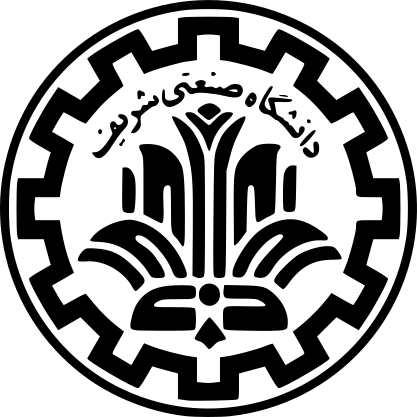
\includegraphics[scale=0.25]{logo.png}\\
		\vspace{0.5cm}
		\begin{Large}
			\textbf{
				Sharif University of Technology\\
				\vspace{0.5cm}
				Computer Science Department\\
			}
		\end{Large}
		\vspace{2.5cm}
		\begin{huge}
			\textbf{
				Advanced Programming Project\\
				 Phase 1\\
				\vspace{1cm}
				Hearthstone\\
			}
		\end{huge}
		\vspace{1.5cm}
		\begin{Large}
			\textbf{
				\\
				\vspace{1cm}
				Amirhossein Afsharrad\\
				\vspace{0.5cm}
				95101077\\
				\vspace{2cm}
				\today
			}
		\end{Large}
		
	\end{center}
	
	\thispagestyle{empty}
\end{titlepage}	

\large
\tableofcontents
\clearpage
\section{Introduction}
In this document we briefly explain all packages and classes implemented for the first phase of the Hearthstone game project. The goal for this phase is to implement the basic structure of the game, so the game is not still ready to be played. You may find all packages and classes attached to this report, or you can check them using the following link on GitHub:
\begin{center}
	\url{https://github.com/AmirAfsharrad/Hearthstone}
\end{center}
The java version of this project is java11 and it has been built using \textit{Gradle}. Apart from java standard packages, only the two following dependencies have been added to the \texttt{build.gradle} file for the \texttt{gson} and \texttt{json} respective packages:
\begin{itemize}
	\item \texttt{compile 'com.googlecode.json-simple:json-simple:1.1.1'}
	\item \texttt{compile group: 'com.google.code.gson', name: 'gson', version: '2.8.5'}
\end{itemize}

\clearpage
\section{How does the project work? - The Big Picture}
In this section we are going to explain how the project works in general. The details of implementation are explained in next sections.\\

To start the game, you need to run the following code:
\begin{lstlisting}[style = javaStyle]
	GameHandler.getGameHandler().runGame();
\end{lstlisting}

The \texttt{GameHandler} class is a singleton class who is responsible for maintaining the general running process of the game. The code above will result in the following code to be run:
\begin{lstlisting}[style = javaStyle]
CLI cli = CLI.getGetCLI();
cli.run();
\end{lstlisting}
The \texttt{CLI} class is also another singleton class which is responsible for the processing of the input commands from the user. \\
After calling the \texttt{cli.run()} method, the key process of the game starts using the following infinite \texttt{while} loop:
\begin{lstlisting}[style = javaStyle]
while (true){
	try {
		currentPlace.defaultResponse();
		command = GetResponseFromUser.getResponse(user);
		currentPlace = currentPlace.runCommand(command, user, currentPlace);
		} catch (Exception e){
			Logger.log(user, "error", Arrays.toString(e.getStackTrace()), true);
	}
}
\end{lstlisting}
In the above loop three tasks are continuously done:
\begin{enumerate}
	\item A default response is given to the user. It depends on the \texttt{currentPlace} which is an object determining where in the game we currently are. For example we could be in the main menu, collections, store, etc. and a default response could be: "You are in the main menu. Where to go?".
	
	\item The process waits until the user enters a command. 
	
	\item The command has to be processed so that two decisions are made:
	\begin{enumerate}
		\item Take appropriate actions such as printing a response or changing user attributes (such as cards, current hero, deck, etc.)
		\item Determine the new \texttt{currentPlace}
	\end{enumerate}
\end{enumerate}

So by inspecting the above code you would conclude that the key method for running the game is the \texttt{runCommand} method called for the \texttt{currentPlace}.\\
In order to gain a better understanding of how this project works, note that there exists an abstract class called \texttt{Place} who has different subclasses such as \texttt{SignInOrSignUp}, \texttt{MainMenu}, \texttt{Collections}, and \texttt{Store}. Each of these classes are singletons since we need one and only one of each place. The \texttt{runCommand} method is also an abstract method of the \texttt{Place} class, so each of the places have to override \texttt{runCommand} for themselves so that they can process the input command from the user and take appropriate actions. The output of this method is also a \texttt{Place} which determines the next place of the game after the command is processed.

Figure \ref{fig01} shows a schematic of how the project works.

\begin{figure}[h!]
	\centering
	\begin{tikzpicture}
	\tikzset{myptr/.style={decoration={markings,mark=at position 1 with %
				{\arrow[scale=3,>=stealth]{>}}},postaction={decorate}}}
		\draw (0,0) rectangle (3,2);
		\draw (0,3) rectangle (3,5);
		\draw [myptr] (-4, 2/3) -- (0,2/3);
		\draw [myptr] (3, 2/3) -- (6,2/3);
		\draw (6.75, 2/3) node {Output};
		\draw [myptr] (0, 4) -- (-1,4) -- (-1, 4/3) -- (0,4/3);
		\draw [myptr] (3,4/3) -- (4, 4/3) -- (4,4) -- (3, 4);
		\draw (1.5,1) node {Run Command};
		\draw (1.5,4) node {Current Place};
		\draw (-2.5,1) node {Command};
		\draw (-5,2/3) circle (1);
		\draw (-5,2/3) node {User};
		\draw (1.5,-3) circle (1);
		\draw (1.5,-3) node {Database};
		\draw [myptr] (1, -1.15-1) -- (1,0);
		\draw [myptr] (2,0) -- (2, -1.15-1);
		\draw (.6,-1.1) node {load};
		\draw (2.4,-1.1) node {save};

	\end{tikzpicture}
	\caption{Schematic of the project structure}
	\label{fig01}
\end{figure}

In the following sections, we explain each package and its classes.




\clearpage
\section{Package \texttt{Cards}}
This package contains classes related to cards of the game. There is an abstract class \texttt{Card} which has three subclasses \texttt{Minion}, \texttt{Spell}, and \texttt{Weapon}. There is also another class called \texttt{CardCreator} which creates a \texttt{Card} object by taking the name of the card as input. The following is a more detailed description of the classes in this package.
\subsection{Class \texttt{Card}}
This class is an implementation for the cards of the game. The class has been declared abstract, since all cards are one of the three subclass types of minion, spell, or weapon and we will not need any direct instances of the abstract type \texttt{Card}. The attributes and methods of this class are as follows:
\subsubsection{Attributes}
\begin{itemize}
	\item \texttt{\textbf{private int mana}}\\
	The mana cost of the card.
	
	\item \texttt{\textbf{private String name}}\\
	The name of the card.
	
	\item \texttt{\textbf{private String rarity}}\\
	The rarity of the card, which is one of the four types: common, rare, epic, or legendary.
	
	\item \texttt{\textbf{private String heroClass}}\\
	The class of hero(es) which could have this card in their deck. It could be Mage, Rogue, Warlock, or neutral.
	
	\item \texttt{\textbf{private String description}}\\
	Description of the card. For now this field is merely a string, but we may need a class for it in future development of the game.
	
	\item \texttt{\textbf{private String type}}\\
	This field determines whether the card is a minion, a spell, or a weapon. Since this class is abstract, one could remove this field and use the \texttt{getClass()} method on the subclasses of \texttt{Card} to know their type, but defining an attribute for type would result in a simpler and more easily-understood code.
\end{itemize}

\subsubsection{Methods}
We shall skip the setters and getters and only describe other methods.
\begin{itemize}
	\item \texttt{\textbf{public int getPrice()}}\\
		This method determines the price of the cards. There could be various methods to determine the price, but in this phase we have simply used the card's rarity for this purpose. The price for common, rare, epic, and legendary cards are 10, 20, 30, and 40 (measured in terms of the game's unit of money) respectively.
		
		\item \texttt{\textbf{public String toString()}}\\
		We have overridden the \texttt{toString()} method to return only the card's name. That is because whenever we need to print a card in our code, we only need to show the card's name. One could tell that we could have used the \texttt{getName()} method and avoided overriding the \texttt{toString()} method, which is correct but we have done so to make our code simpler and better-understood.
		
		\item \texttt{\textbf{public boolean equals(Object object)}}\\
		We have overridden the \texttt{equals} method in order to be able to check if two cards are the same. The important point is that for two cards, we know from the game structure that only comparing the names suffices to check whether they are the same or not, and that is what we have done in \texttt{equals} method. This is because the cards in this game have unique names and there are no pairs of cards having the same names but different features.
\end{itemize}

\subsection{Classes \texttt{Minion}, \texttt{Spell}, and \texttt{Weapon}}
These three classes are the children of \texttt{Card} who have a few (or none for \texttt{Spell}) more attributes. These attributes are listed below:
\begin{itemize}
	\item \texttt{\textbf{private int attackPower}}\\
	This is the attack power of the card, which is a shared attribute of minions and weapons.
	
	\item \texttt{\textbf{private int hp}}\\
	This is the health point field, which is only an attribute of the minion class and the other two types do not need a health point.
	
	\item \texttt{\textbf{private int durability}}\\
	This is a specific feature of weapons, which determines how many times a weapon could be used. The other two types of cards do not need such a feature.
	
\end{itemize}

\subsection{Class \texttt{CardCreator}}
The primary goal of this class is to create a card by getting the card name in the input. As it was mentioned before, the cards are uniquely determined by their names and there are no pairs of cards with the same name but different features. This would suggest us to even remove the card classes and only work with cards as strings, but this will result in a lot of problems in future when we are going to use cards in the game (although this approach would make this phase of the project much simpler since we wouldn't have to convert card objects to strings and vice versa for saving and loading as they would have been mere strings). 

As a result of this feature, we can create a card by just knowing its name and looking in a database of cards' features. As explained in sections \ref{initialization}, we have such database saved in the file \texttt{All Cards.json}. So This class is only responsible to have a method to take the card name, look into the database and extract other features of that specific card, and create an object of the card. That is what happens in the following methods:
\begin{itemize}
	\item \texttt{\textbf{private static Minion createMinion(JSONObject cardObj)}}\\
	
	This method takes the card to be created as a \texttt{JSONObject} and extracts the features of the card and finally creates a \texttt{Card} object. Note that this method is specified for minions. There are two more similar methods responsible for spells and weapons. Before going to the next methods, there are two important points to be stated: First, this method is private, and that is because this method (along with the next two who do the same thing for spells and weapons) are used by the public method \texttt{createCard} which is is explained below. Second, the input of this method is a \texttt{JSONObject}, and that is because our database file is a JSON file. This will also be more clear after going through the method \texttt{CreateCard}.
	
	\item \texttt{\textbf{private static Spell createSpell(JSONObject cardObj)}}\\
	Similar as the previous method but for spell cards.
	
	\item \texttt{\textbf{private static Weapon createWeapon(JSONObject cardObj)}}\\
	Similar as the previous method but for weapon cards.	
	
	\item \texttt{\textbf{public static Card createCard(String cardName)}}\\
	This method, as we mentioned before, is the only public method of this class which creates a card by taking its name as a string in the input. It first opens the JSON database file and reads the list of all cards as a \texttt{JSONArray}, then looks for the card with the specified name. Then it looks at the type of the card and decides which of the three previous methods to call. Now it is more clear why we set the input type of the previous methods to \texttt{JSONObject}, since in this method we have a \texttt{JSONObject} extracted from a \texttt{JSONArray} which needs to turn into a \texttt{Card} object.
	
\end{itemize}

\clearpage
\section{Package \texttt{Heroes}}
This package contains the implementation of all heroes of the game. There are three types of heroes to be implemented in Hearthstone: Mage, Rogue, and Warlock. For each type, we have designed a class, and also there is an abstract class \texttt{Hero} which is extended by all three real hero types.
\subsection{Class \texttt{Hero}}
As it was just mentioned, this is an abstract class who is responsible for the general structure of a hero. The fields and methods of this class are explained below. We skip the setters and getters since their function is obvious.
\subsubsection{Attributes}
\begin{itemize}
	\item \textbf{\texttt{protected int defaultHp}}\\ This is the default value for the hero's health point. It has been set to 30 as the project instructions asked for, but it could be set to any other value. It's access modifier has been set to \texttt{protected} since other subclasses of \texttt{Hero} need to know this value.
	
	\item \textbf{\texttt{private int hp}}\\ This is the health point of the hero, which varies during the game-play.
	
	\item \textbf{\texttt{private String type}}\\
	 This field is responsible to determine which type of hero (Mage, Rogue, or Warlock) an object of type \texttt{Hero} is. Actually we could do without this feature since \texttt{Hero} is an abstract class and the objects to be instantiated are of the types \texttt{Mage}, \texttt{Rogue}, or \texttt{Warlock}; and we could run the \texttt{getClass()} method on these objects to know their hero type. However creating a string field of type would result in a simpler and better-looking code.
	
	\item \textbf{\texttt{private String heroPower}}\\
	This is one of the features for the heroes, about which there is almost nothing implemented in the first phase. As a result, it has been defined in this class as a string field which only contains the description of the hero power. We may define a new class for hero power in future if we need to.
	
	\item \textbf{\texttt{private  specialPower}}\\
	About this field everything is similar to \texttt{heroPower}. We may design a separate class for \texttt{heroPower} but for now a simple string would suffice.
	
	\item \textbf{\texttt{private ArrayList<Card> deck}}\\
	This field is an \texttt{ArrayList} of cards, which holds the deck for the hero.
	
	\item \textbf{\texttt{private int deckCapacity}}\\
	This is the maximum number of cards heroes can have in their deck. It has been set to a default value of 15 according to the project instructions.
	
	\item \textbf{\texttt{private int maxRepetitiveCardsInDeck}}\\
	This item is the maximum number of the same card that a hero can have in the deck. The default value for this parameter is set to 2 according to the project instructions, but it could easily be modified if needed.	
\end{itemize}

\subsubsection{Methods}


\begin{itemize}
	\item \textbf{\texttt{public int getNumberOfCardsInDeck()}}\\
	This method returns the number of the cards present in the hero's deck. This method is useful when the game controller wants to check whether a card could be added to the hero's deck or not.
	
	\item \textbf{\texttt{public int getHowManyOfThisCardInDeck(Card card)}}\\
	This method takes a \texttt{Card} object as the input and returns how many of that card exists in the hero's deck. It is used to prevent the user from adding more than the specified limit \texttt{maxRepetitiveCardsInDeck} of the same card to a hero's deck.
	
	\item \textbf{\texttt{public ArrayList<String> getDeckAsArrayOfString()}}\\
	This method returns the hero's deck as an \texttt{ArrayList} of Strings. We need to transform the cards to string in order to be able to save them as JSON objects.
	
	\item \textbf{\texttt{public JSONObject getJson()}}\\
	This method returns a \texttt{JSONObject} containing all attributes of a hero which we need to save when a user logs out of his or her account.
	
\end{itemize}

\subsection{Classes \texttt{Mage}, \texttt{Rogue}, and \texttt{Warlock}}
These three classes are children of the \texttt{Hero} class who inherit all its fields and methods. They are very similar so we explain them in the same section. These classes need no more fields than their superclass, and they are only different in \texttt{type}, \texttt{heroPower}, and \texttt{specialPower}. These differences have been handled in the constructors of each of the three \texttt{Hero} subclasses. As a result one might think of not creating three different classes for hero types and only using a single hero class. This idea could also work properly but we shall see that having three separate classes has resulted in more simplicity in our design. The only other thing to be mentioned is the \texttt{toString()} method which is overridden for these three classes and returns their \texttt{type}. It is obvious that we could avoid overriding \texttt{toString()} method and user \texttt{hero.getType()} whenever needed, but we have done so for simplicity.

\subsection{Class \texttt{HeroCreator}}
This class contains only a single static method:
\begin{itemize}
	\item \textbf{\texttt{public static Hero createHeroFromJson(JSONObject heroJsonObject)}}\\
	It returns a \texttt{Hero} object after taking a \texttt{JSONObject} in the input. This method actually does the reverse of the \texttt{JSONObject getJson()} method in \texttt{Hero} class who would turn a \texttt{Hero} into a \texttt{JSONObject}. These two work as complements for save and load processes.
	
\end{itemize}

\clearpage
\section{Package \texttt{UserHandle}}
This package is responsible for users and their data. It plays the key role in save and load processes, and it also defines the key object \texttt{User}. We shall review the two important classes of this package in this section.

\subsection{Class \texttt{User}}
This class is responsible for keeping all the data of a user who is playing the game. The fields and methods of the \texttt{User} object are as follows:

\subsubsection{Attributes}
\begin{itemize}
	\item \texttt{\textbf{private int id}}\\
	The user ID which is unique among all users ever playing the game (even if they remove their account).
	
	\item \texttt{\textbf{private String name}}\\
	The name that user registers his or her account with.
	
	\item \texttt{\textbf{private String password}}\\
	The password of the user. Note that, as it shall be discussed in more details later, the game does not store the explicit password of any user, but it stores the hashed form of the passwords using SHA256 hashing method.
	
	\item \texttt{\textbf{private int gold}}\\
	The amount of gold (money) a user has (which could be used in the store).
	
	\item \texttt{\textbf{private ArrayList<Card> cards}}\\
	The list of all the cards a user owns. For a newly registered user this list consists of ten cards. The method \texttt{initializeCardsAndHeroesAsDefault} is responsible for initializing the cards.
	
	\item \texttt{\textbf{private ArrayList<Hero> heroes}}\\
	The list of all the heroes a user owns. For a newly registered user this list only consists of Mage.
	
	\item \texttt{\textbf{private int currentHeroIndex}}\\
	A user must always be aware of his or her current hero. One way to do so was to create a \texttt{Hero} object as \texttt{currentHero}, but for the sake of code simplicity we used another approach. We only keep the index of the current hero as an index of the \texttt{ArrayList} \texttt{heroes}. This makes many things simpler. One important example is that if we created an independent field for \texttt{currentHero}, we always had to take care of updating the respective hero in the \texttt{heroes} list when a change occurred to the \texttt{currentHero}, but working with only an index lets us work directly with the \texttt{heroes} list and modify any of the heroes in that list which is being used as the current hero.
	
	\item \texttt{\textbf{private boolean loggedIn}}\\
	For any user we would need to know whether it is logged in as the current user or not. This field keeps a \texttt{boolean} to answer this question.
	
	
\end{itemize}

\subsubsection{Methods}
\begin{itemize}
	\item \texttt{\textbf{public void setCurrentHero(String heroName)}}\\
	This method takes a hero (or hero name) and modifies \texttt{currentHeroIndex} to change and set the current hero.
	
	\item \texttt{\textbf{public void copy (User user)}}\\
	This method takes a \texttt{User} object in the input and copies all its values to the current user. We had to write this method since we needed to modify a \texttt{User} object inside a method, while the real object was outside the method body. As a result, we had to change the attributes one by one and we could not only change the reference since what we have inside the method is not the original reference but a copy of that.
	
	\item \texttt{\textbf{public boolean hasHero(String hero)}}\\
	This method simply returns a \texttt{boolean} to show whether a user has a hero or not.
	
	\item \texttt{\textbf{public boolean hasCard(String cardName)}}\\
	This method simply returns a \texttt{boolean} to show whether a user has a card or not.	
	
	\item \texttt{\textbf{public void addHero(Hero hero)}}\\
	This method adds a hero to the user's list of heroes.
	
	\item \texttt{\textbf{public ArrayList<String> getHeroesAsArrayOfString()}}\\
	This method returns the list of a user's heroes as a string list. This might come in handy when we want to know all the heroes a user has, while we could do without this method only using \texttt{hasHero} method.
	
	\item \texttt{\textbf{public void initializeCardsAndHeroesAsDefault()}}\\
	This method is responsible for initializing the cards and heroes of a user. The heroes list is set to a default list only containing a Mage, and the card list is initialized to 10 cards which could be accessed in a file named \texttt{Default User Cards.txt}. This file is generated with the methods of the package \texttt{Initialization} explained in the section \ref{initialization}.
	
	\item \texttt{\textbf{public ArrayList<String> getCardsAsArrayOfString()}}\\
	This method does the same thing as \texttt{getHeroesAsArrayOfString()} but for the cards.
	
	\item \texttt{\textbf{public void addCard(Card card)}}\\
	This method adds a card to the user's list of cards.
	
	\item \texttt{\textbf{public void removeCard(Card card)}}\\
	This method removes a card from the user's list of cards.
		
	\item \texttt{\textbf{public boolean isForSale(Card card)}}\\
	This method is responsible to answer the questions "Can the user sell this card?". This actually means that this method has to check whether any of the user's heroes have this card in their decks or not. If the card is not present in any of the heroes' decks, the user can sell it. If not, he or she has to first remove it from those decks. This method is used in the warning system of the store where one wants to sell or buy cards.
	
	\item \texttt{\textbf{public JSONArray getHerosJsonArray()}}\\
	This method returns a \texttt{JSONArray} containing the data of all heroes of a user. This \texttt{JSONArray} is used to save (and later load) the needed data for a user's heroes.
	
	\item \texttt{\textbf{public String toString()}}\\
	We have also overridden the \texttt{toString()} method for \texttt{User} object to print its attributes when needed.
	
\end{itemize}

\subsection{Class \texttt{UserDataHandler}}
This class is simply the interface of the game and the data that is saved outside the program. There are four main methods in this class for adding, saving, loading, and removing user accounts. There are also some other private methods who help the four main methods perform in a good way. These methods are as follows:
\begin{itemize}
	\item \texttt{\textbf{private static int getUserIndexIfExists(String userName)}}\\
	This method returns the ID of a given user if it is an active user (i.e. a user which has been created and not removed yet). This could help the system load the saved data. Also, it has been declared private since only other methods in this class need to use it.
	
	\item \texttt{\textbf{private static boolean userMatchCheck(String userName, JSONObject user)}}\\
	This method does a very simple task. It takes a \texttt{JSONObject} and a string to check whether the object has the same name as the string or not.
	
	\item \texttt{\textbf{public static User add(User user)}}\\
	This method adds a user to the system if there is no active user with the same user name. It reads the previously saved data from the \texttt{users.json} file, adds a new user to the end of the file, and saves it again.
	
	\item \texttt{\textbf{public static User load(String userName, String password)}}\\
	This method loads the needed data when a user who has previously created an account wants to sign in. It reads data from \texttt{users.json} file after checking whether the account exists and the entered password matches the saved password. As previously stated, the passwords saved in the file \texttt{users.json} are hashed, so to check the input password, this method calculates its hash and compares it with what was saved in the database file.
	
	\item \texttt{\textbf{public static void save(User user)}}\\
	When a user decides to sign out of the game, this method has to save its data. It acts similar to \texttt{add} method. It opens the \texttt{users.json} file and loads its data into a \texttt{JSONArray}, finds the user in that array and replaces its data with the updated data. After that it writes the \texttt{JSONArray} into the database file again and the saving process in complete.
	
	\item \texttt{\textbf{public static void remove(String userName, String password)}}\\
	As we mentioned before, user IDs are unique even after the user is removed. So the \texttt{remove} method only changes an attribute of the user in the data file by adding the exact time of deletion of the account. After this happens, one is allowed to create a new user with the same name as the removed user. This method updates the \texttt{users.json} file and adds the deletion timestamp to it in a very similar manner as the \texttt{save} method works.
	
\end{itemize}

\clearpage
\section{Package \texttt{Places}}
\subsection{Class \texttt{Place}}
This game contains different places. The user is permitted to do certain things in each place. For this phase of the project, we have defined four different places, each of which is taken care of by a separate class. Class \texttt{Place} is the supperclass to all places and it has been declared abstract since all real places are the instances of its subclasses.

\subsubsection{Attributes}
\begin{itemize}
	\item \texttt{\textbf{private HashMap<String, String> instructions}}\\
	This field is a \texttt{HashMap}, whose keys are the valid commands a user can enter in this place. The values of this \texttt{HashMap} are the instructions for each command. We use this field whenever the user enters the command \texttt{hearthstone --help}.
	
	\item \texttt{\textbf{private String instructionsPath}}\\
	This is the address of the file in which the valid commands and their instructions are saved. We use methods from the package \texttt{Initialization} (explained in section \ref{initialization}) to generate these files.
\end{itemize}

\subsubsection{Methods}
\begin{itemize}
	\item \texttt{\textbf{public void loadInstructions()}}\\
	This method reads the JSON file from the path \texttt{instructionsPath} and loads its data into the \texttt{HashMap} \texttt{instructions}. We run this method for each subclass of \texttt{Place} in the constructor (with its specific \texttt{instructionsPath}).
	
	\item \texttt{\textbf{public abstract Place runCommand(String command, User user, Place currentPlace)}}\\
	We always need to process the input from the user during the run time of the game. In each place, there must be a \texttt{runCommand} method to do this job. That is why we have declared it as an abstract method, so it would be implemented in each of the subclasses according to the set of valid commands in that specific subclass.\\
	We have set the output type of this method a \texttt{Place} so that it will return the place \textit{after the command is processed} as commands could obviously result in a change of place during the game.
	
	\item \texttt{\textbf{public abstract void defaultResponse()}}\\
	When the game is running, each place needs a default response (for example "You are in main menu. Where to go?") to show to the user. This method is responsible to produce this response and it is declared abstract so that all places implement it for themselves.
\end{itemize}

\subsection{Classes \texttt{SignInOrSignUp}, \texttt{MainMenu}, \texttt{Collections}, and \texttt{Store}}
For this phase of the project, there are four places in the game. For each of these places we have designed a separate class. The most important task for each class is to override the method \texttt{runCommand}. In fact, the key process which makes the CLI a good interface is what happens inside these \texttt{runCommand} methods. They are responsible for processing the user input and return appropriate outputs.\\
We are not going to explain the code in each of these methods in this document, but they are generally in the form of a big \texttt{switch case} who checks different cases of the input command.\\
Also an important point is that all these four classes have been designed using the \textit{singleton} design pattern since for each place, there has to be one and only one instance of that place.


\clearpage
\section{Package \texttt{GameHandler}}
This package contains a class named \texttt{GameHandler} and another internal package \texttt{CLI}. They are explained in this section.
\subsection{Class GameHandler}
This class is responsible for general operation of the game. That is why it has been created using the \textit{singleton} design pattern. There has to be one and only one game handler it the game.

\subsubsection{Attributes}
\begin{itemize}
	\item \texttt{\textbf{private static GameHandler gameHandler}}\\
	We need a \texttt{GameHandler} object for the singleton design pattern.
	
	\item \texttt{\textbf{private HashMap<String, Card> allCards}}\\
	This field is the set of all cards in the game. We could do without this field and create a card whenever needed using the \texttt{CardCreator.createCard} method, but since this method needs to read from a file, it will take much more time if it is going to be called many times during the game. To avoid this problem, we only do this once and create an instance of all possible cards and save them in this field, and use the cards whenever needed. 
	
	\item \texttt{\textbf{private ArrayList<String> allCardNames}}\\
	This field keeps the names of all game cards in an \texttt{ArrayList} to be accessed whenever needed. It is actually used when listing all possible cards a user can buy in the store.
	
	\item \texttt{\textbf{private String path}}\\
	This is the address of the cards database from which the information needed for initializing \texttt{allCards} and \texttt{allCardNames} is extracted.
\end{itemize}

\subsubsection{Methods}
\begin{itemize}
	\item \texttt{\textbf{public void refreshCardsDatabase()}}\\
	This method uses the address in \texttt{path} to initialize or refresh \texttt{allCards} and \texttt{allCardNames}. In general, it is run once inside the constructor of the class.
	
	\item \texttt{\textbf{public Card getCard(String cardName)}}\\
	This method returns a \texttt{Card} object by taking the name of the desired card at the input.
	
	\item \texttt{\textbf{public static void runGame()}}\\
	This method gets the instance of CLI (which is a singleton class) and runs the \texttt{run()} method of the CLI, so the game shall run. One could run the game and start playing by just calling \texttt{GameHandler.getGameHandler().runGame()}.
	
\end{itemize}

\subsection{Package \texttt{CLI}}
This package is responsible for the command line interface of the game. In contains three small but important classes.
\subsubsection{Class \texttt{CLI}}
This is a singleton class who is responsible to maintain the command line interface. Apart from the single \texttt{CLI} object and its getter, this class only contains one method:
\begin{itemize}
	\item \texttt{\textbf{public void run()}}\\
	This method uses an infinite \texttt{while} loop and performs the following three steps:
	\begin{enumerate}
		\item Run a default response for the current place of the game.
		\item Get a command from the user.
		\item Process the command and do the appropriate task.
	\end{enumerate}
	Doing these three steps in an infinite loop is what makes the game work.
\end{itemize}

\subsubsection{Class \texttt{RespondToUser}}
This is a simple class which gives the desired response to the user. For this phase it only contains a simple print, but it needs further development for the next phases (graphical interface). It also uses the output command for logging. This simple method has the following signature:
\begin{itemize}
	\item \texttt{\textbf{public static void respond(Object message, User user)}}\\
	Note that it has two inputs, a message and a user. The message is clearly taken to be printed. The user, on the other hand, is only taken as an input for the logging process and has nothing to do with the on-screen printing.
\end{itemize}

\subsubsection{Class \texttt{getResponseFromUser}}
This class has a single method which is overloaded with four different signatures:
\begin{itemize}
	\item \texttt{\textbf{public static String getResponse()}}
	\item \texttt{\textbf{public static String getResponse(Object message)}}
	\item \texttt{\textbf{public static String getResponse(User user)}}
	\item \texttt{\textbf{public static String getResponse(Object message, User user)}}
\end{itemize}
These methods are simply responsible for taking the input command from the user, but they sometimes use that command for logging, and they sometimes print an output simultaneously. As a result, four different signatures (do the logging or not, and print something before getting the input or not) exist for this method.\\

\clearpage
\section{Package \texttt{Logger}}
This package is responsible for logging the game and has a single class \texttt{Logger}.
\subsection{Class \texttt{Logger}}
\subsubsection{Attributes}
\begin{itemize}
	\item \texttt{\textbf{private static String defaultPath}}\\
	This is the only attribute of this class which stores the default path for saving the logs.
\end{itemize}

\subsubsection{Methods}
\begin{itemize}
	\item \texttt{\textbf{public static void InitializeNewUserLogFile(User user)}}\\
	This method creates a new log file for a new user and writes the header of the log file using the name and ID of the user.
	
	\item \texttt{\textbf{public static void log(User user, String event,\\ String eventDescription, boolean... systemLog)}}\\
	This method takes a \texttt{User} as input to know which user's log file is to be updated. It then takes two more inputs \texttt{event} and \texttt{eventDescription} and writes them in the user's log file. Also there is another input \texttt{systemLog} which is an arbitrary \texttt{boolean} input that determines whether to register a system log or not. System logs are explained below (the \texttt{systemLog} method).
	
	\item \texttt{\textbf{public static void terminateUserLog(User user)}}\\
	This method is called whenever a user is removed. It opens the user's log file and updates the deletion time in the file.
	
	\item \texttt{\textbf{public static void systemLog(String event, String eventDescription)}}\\	
	Apart from the log files for each user, there is another log file named \texttt{hearthstone.log} in which general occurrences of the game are logged. These include user acts and system errors. This method is responsible to log these events.
\end{itemize}


\clearpage
\section{Package \texttt{Utilities}}
This package contains some helper classes which are needed in different other classes. Note that some of the methods in this package have been taken from online websites whose names the author has unfortunately forgotten.
\subsection{Class \texttt{FileHandler}}
This class contains some useful methods for working with files. They are listed below:
\begin{itemize}
	\item \texttt{\textbf{public static List<String> readFileInList(String path)}}\\
	This method reads a text file (line by line) into a list.
	
	\item \texttt{\textbf{public static String readFileInString(String path)}}\\
	This method reads a text file into a single string.
	
	\item \texttt{\textbf{public static void writeListIntoFile(List list, String path)}}\\
	This method writes a list into a text file (line by line).
	
	\item \texttt{\textbf{public static void writeStringIntoFile(String text, String path)}}\\
	This method writes a string into a text file.
	
	\item \texttt{\textbf{public static void writeJsonObjectToFile(JSONObject jsonObject, String path)}}\\
	This method writes a \texttt{JSONObject} into a JSON file.
	
	\item \texttt{\textbf{public static void writeJsonArrayToFile(JSONArray jsonArray, String path)}}\\
	This method writes a \texttt{JSONArray} into a JSON file.
	
	\item \texttt{\textbf{public static JSONObject getJsonObjectFromFile(String path)}}\\
	This file reads a \texttt{JSONObject} from a JSON file.	

	\item \texttt{\textbf{public static JSONArray getJsonArrayFromFile(String path)}}\\
	This file reads a \texttt{JSONArray} from a JSON file.

	
	
\end{itemize}
\subsection{Class \texttt{SHA256Hash}}
This class has a single method which returns the hash of an input string using the SHA256 hashing method. The method's signature is as follows:
\begin{itemize}
	\item \texttt{\textbf{public static String getHashSHA256(String inputString)}}
\end{itemize}

\subsection{Class \texttt{TextProcessingTool}}
This class has three simple methods for text processing. They are specifically designed for the \texttt{runCommand()} methods in \texttt{Place} subclasses who are responsible to process the user input command.

\begin{itemize}
	\item \texttt{\textbf{public static boolean stringFirstWordMatch(String mainString,\\ String doesMatchString)}}\\
	This method checks whether an input command starts with a specific word or not.
	
	\item \texttt{\textbf{public static boolean isInBrackets(String string)}}\\
	This method checks whether or not a string is bracketed, i.e., in the form \texttt{[inputString]} where \texttt{inputString} could be any arbitrary string.
	
	\item \texttt{\textbf{public static String unBracket(String string)}}\\
	This method returns the unbracketed version of a bracketed string.
	
\end{itemize}


\clearpage
\section{Package \texttt{Initialization}} \label{initialization}
This package is responsible for some initialization tasks which need to be done once before the first ever run of the game. They will not be needed unless database files are lost or a change in game structure has taken place.

\subsection{Class \texttt{CardsDataCreator}}
This class has one important method with the following signature which creates a JSON file containing the data of all cards in the game.
\begin{itemize}
	\item \texttt{\textbf{public static void createCardsData()}}
\end{itemize}

\subsection{Class \texttt{DefaultUserCardsDataCreator}}
This class has a single method to create a text file containing a list of default cards a user has when his or her account has just been created. For this phase it contains ten randomly selected (but fixed) cards. The method signature is as below:
\begin{itemize}
	\item \texttt{\textbf{public static void createDefaultUserCardsData()}}
\end{itemize}

\subsection{Class \texttt{PlaceDataCreator}}
This class is responsible for creating JSON files for each of the four places in the game, each of the files containing the set of valid commands and their instructions. As mentioned before, this data is used to respond to user's \texttt{hearthstone --help} command. There are five methods in this class, four of which responsible for creating the command instruction files for each of the four places, and a fifth method which runs all previous four:
\begin{itemize}
	\item \texttt{\textbf{public static void initSignInOrSignUp(String... path)}}
	\item \texttt{\textbf{public static void initMainMenu(String... path)}}
	\item \texttt{\textbf{public static void initCollections(String... path)}}
	\item \texttt{\textbf{public static void initStore(String... path)}}
	\item \texttt{\textbf{public static void initAllPlaces()}}
\end{itemize}






\end{document}


